% Setup - do not change
\documentclass[11pt]{article}
\usepackage[top=0.9in, left=0.9in, bottom=0.9in, right=0.9in]{geometry} 
\usepackage{parskip}

\usepackage[english]{babel}
\usepackage[utf8]{inputenc}
\usepackage{amsmath,amsthm,amssymb,graphicx,pdfpages,lipsum,hyperref}
\usepackage[none]{hyphenat}
\usepackage{csquotes}

\setlength\parindent{0pt}
%%%%%%%%%%%%%%%%%%%%%%%%%%%%%%%%%%%%%%%%%%%%%%%%%%%%%%%%%%%%%%%%%%%
% add other packages here if required

\usepackage[export]{adjustbox}

%% Bibliography are specified in this file. You can also choose inline bib style if you want to. But make sure your citation style is consistent (and proper)
% For more details on citation: https://library.unimelb.edu.au/recite
\usepackage[sorting = none]{biblatex}
\addbibresource{references.bib}

%%%%%%%%%%%%%%%%%%%%%%%%%%%%%%%%%%%%%%%%%%%%%%%%%%%%%%%%%%%%%%%%%%% the '%' symbol denotes comments

% Begin document creation
% DELETE THE \lipsum PLACEHOLDERS WHEN YOU BEGIN
\title{\textbf{Applied Data Science (MAST30034) Project 1: Quantitative Analysis} \\ Quantitative Analysis Of The New York City Taxi Data}
\author{
Yuhao Zhai\\
Student ID: 1067899 \\
%% Replace the link with your github repo
% 1. Remember to escape underscore in the link.
% 2. Remember to include the commit you want to submit in the link
\href{https://github.com/NimitzZ001/projectone}{Github repo with commit}
}

\begin{document}
\maketitle

\section{Introduction}
% Link to a 30 min tutorial if you require revision: https://www.overleaf.com/learn/latex/Learn_LaTeX_in_30_minutes

In New York City, taxicabs come in two varieties: yellow and green; they are widely recognizable symbols of the city. Taxis painted yellow (medallion taxis) are able to pick up passengers anywhere in the five boroughs. Those painted apple green (street hail livery vehicles, commonly known as "boro taxis"), which began to appear in August 2013, are allowed to pick up passengers in Upper Manhattan, the Bronx, Brooklyn, Queens (excluding LaGuardia Airport and John F. Kennedy International Airport), and Staten Island. Both types have the same fare structure. Taxicabs are operated by private companies and licensed by the New York City Taxi and Limousine Commission (TLC). It also oversees over 40,000 other for-hire vehicles, including "black cars", commuter vans, and ambulettes.\cite{Taxis}.
Taxicabs are the only vehicles that have the right to pick up street-hailing and prearranged passengers anywhere in New York City. By law, there are 13,587 taxis in New York City and each taxi must have a medallion affixed to it. Medallions are auctioned by the City and are transferrable on the open market by licensed brokers.\cite{YellowCab}. It is important for us to find out the how weather effect the New York City taxi business.  


% You can have \section{}, \subsection{}, and \subsubsection{}
\section{Preprocessing, Analysis, and Geospatial Visualisation}

\subsection{Data Selection}

\subsubsection{Yellow Taxi Trip Records }
In this project, we use yellow taxi trip data for the year 2019 January April, July, and October. Since these 4 months represent the four seasons of the New York City. Which can use for weather analysis.  The data set can be downloaded from from the New York City Taxi and Limousine Commission. The data set has 18 columns: such as pick-up and drop-off dates/times, pick-up and drop-off locations, journey distances, all kinds of fares, fares types, payment types, and driver-reported the number of passengers. 


\subsubsection{weather}
The weather data I use is from kaggle New York City Weather Data 2019.This dataset was gathered to be used in the Big Data Derby 2022 competition. However, it can obviously be used for any other purposes. Horses are affected by weather conditions, so knowing the day's temperature, snowfall, precipitation, etc will definitely be useful.Weather data collected from the National Weather Service. It contains daily data from all days in 2019. It contains for each day the minimum temperature, maximum temperature, average temperature, precipitation, new snow fall, and current snow depth. The temperature is measured in Fahrenheit and the depth is measured in inches. T means that there is a trace of precipitation.\cite{kaggle}

\subsubsection{Taxi Zone data}
The taxi zone data also downloaded \cite{TaxiZone}. This data got each taxi zones geometric information. Also with the Taxi Zone Look Up Table file contains TLC taxi zone location IDs, location names, and each zone corresponding boroughs.

\subsection{Preprocessing}

It approximately got 28696876 trip records for 2019 year 4 months data set with 19 columns of attributes. The data takes 4.1G memory. By changing the datatypes we reduce the data memory usage.

\subsubsection{Data Cleaning}

After we reduce the memory usage, we check the missing value in the yellow taxi data set.
151810 values are missing for passenger\_count, RatecodeID, store\_and\_fwd\_flag features. 5008025 missing values for the congestion\_surcharge feature. According to the feature context, I am able to filter out some error like the distance can't be negative. Finally, the PULocationID and DOLocationID should within NYC taxi zone.\cite{TaxiZone}


Next, in figure \ref{fig:image1} and in figure \ref{fig:image2},we plot the data distribution.

\begin{figure}[!h]
    % change the scale multiplier to make the figures smaller or larger
    \centering
    \adjincludegraphics[height=7cm,clip]{plots/p1.png}
    % \includegraphics[width=\textwidth]{download.png}
    % this ensures your figures are centered where possible
    \caption{trip distance distribution} % refer to this image as (Figure 1)
    \label{fig:image1}
\end{figure}

\begin{figure}[!h]
    % change the scale multiplier to make the figures smaller or larger
    \centering
    \adjincludegraphics[height=7cm,clip]{plots/p2.png}
    % \includegraphics[width=\textwidth]{download.png}
    % this ensures your figures are centered where possible
    \caption{total amount distribution} % refer to this image as (Figure 1)
    \label{fig:image1}
\end{figure}

\subsubsection{Feature Engineering}

The difference between pickup and drop-off time is a useful information for us to know the  period of each trip. The features like tpep\_pickup\_datetime, tpep\_dropoff\_datetime, store\_and\_fwd\_flag that are no longer the features we mainly focus on, these features are dropped. Finally, I select the date in the 4 months of both taxi and weather dataset.

\subsection{Geospatial Visualisation}
\subsubsection{Geospatial and Time Analysis}

These 4 months the total amount of activity in New York City is show. In figure \ref{fig:image3}, The brighter and yellow regions indicate that there are exits more taxi activity. In Manhattan it got most pickups and drop-off activities.

\begin{figure}[!h]
    % change the scale multiplier to make the figures smaller or larger
    \centering
    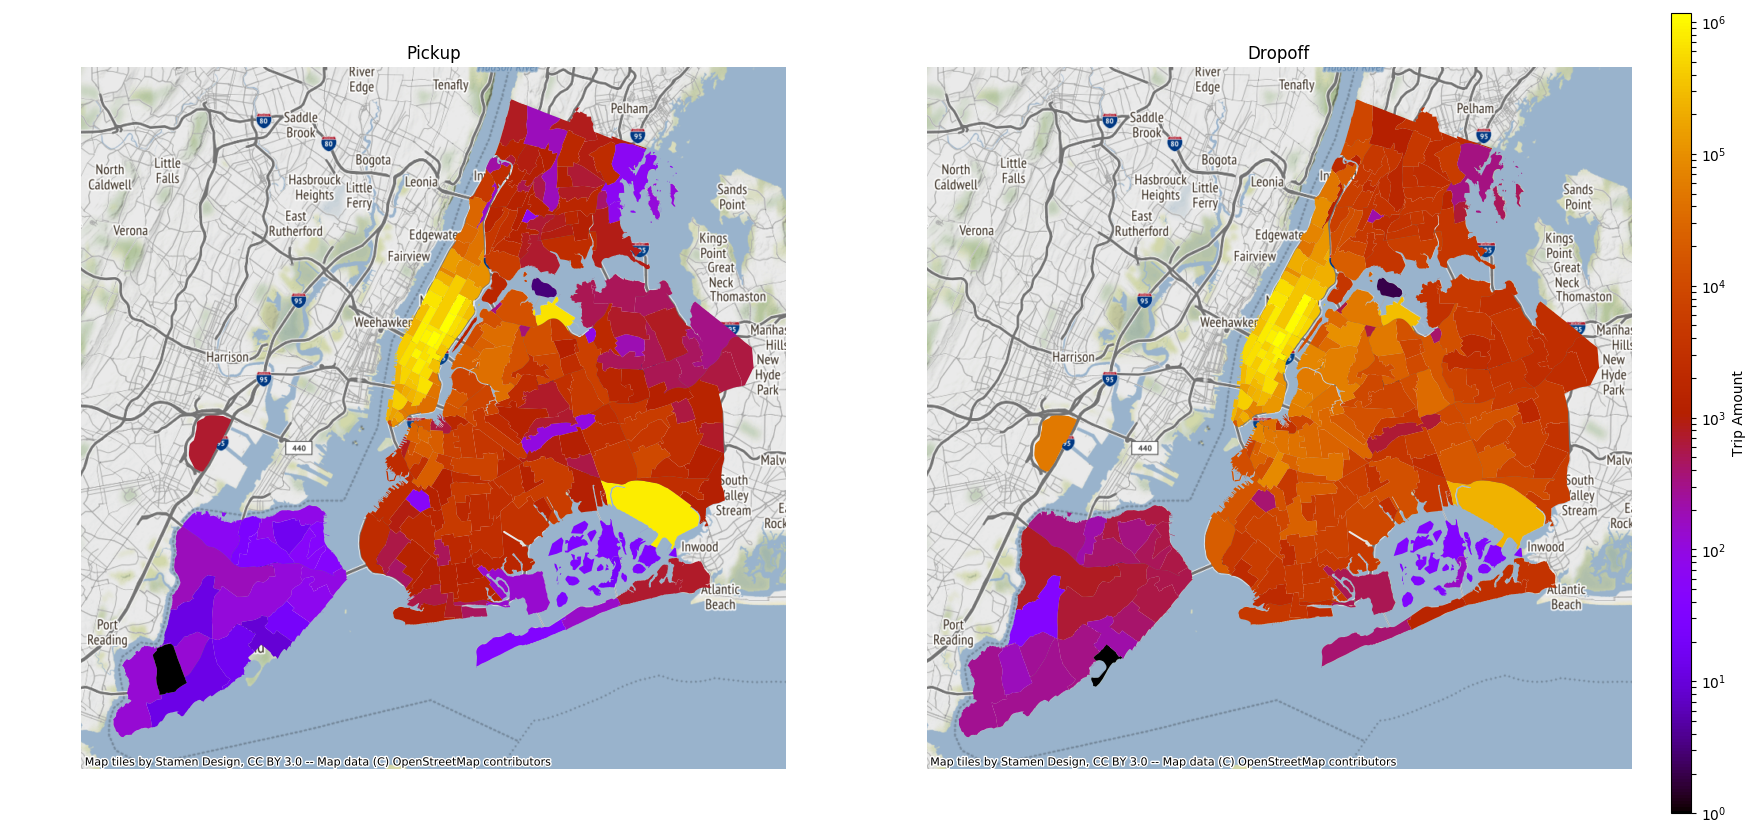
\includegraphics[width=0.8\textwidth]{plots/p3.png}
    % \includegraphics[width=\textwidth]{download.png}
    % this ensures your figures are centered where possible
    \caption{Taxi Pickup Frequency} % refer to this image as (Figure 1)
    \label{fig:image2}
\end{figure}

\subsubsection{Weather Impact}
In this section we investigate how weather affects the taxi bussiness. The following scatter plots shows the weather Average temperature of the day in F versus different data features like 'passenger\_count','trip\_distance','tip\_amount','period', 'total\_amount'. 

\begin{figure}[!h]
    % change the scale multiplier to make the figures smaller or larger
    \centering
    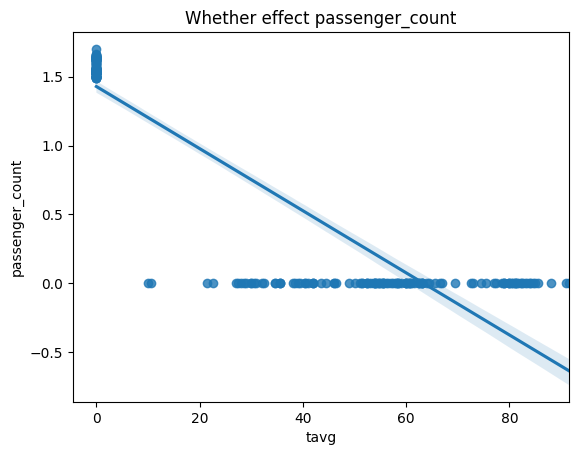
\includegraphics[width=0.5\textwidth]{plots/p4.png}
    % \includegraphics[width=\textwidth]{download.png}
    % this ensures your figures are centered where possible
    \caption{Weather Impact passenger count} % refer to this image as (Figure 1)
    \label{fig:image3}
\end{figure}

\begin{figure}[!h]
    % change the scale multiplier to make the figures smaller or larger
    \centering
    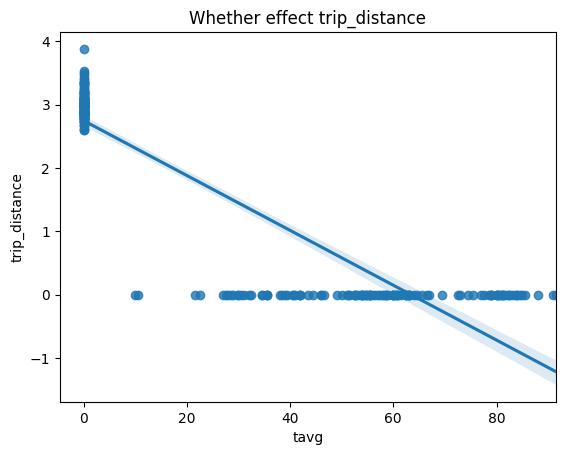
\includegraphics[width=0.5\textwidth]{plots/p5.png}
    % \includegraphics[width=\textwidth]{download.png}
    % this ensures your figures are centered where possible
    \caption{Weather Impact trip distance} % refer to this image as (Figure 1)
    \label{fig:image3}
\end{figure}

\begin{figure}[!h]
    % change the scale multiplier to make the figures smaller or larger
    \centering
    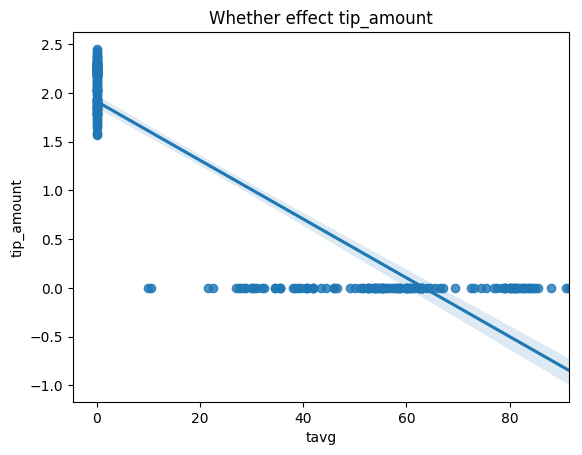
\includegraphics[width=0.5\textwidth]{plots/p6.png}
    % \includegraphics[width=\textwidth]{download.png}
    % this ensures your figures are centered where possible
    \caption{Weather Impact tip amount} % refer to this image as (Figure 1)
    \label{fig:image3}
\end{figure}


\begin{figure}[!h]
    % change the scale multiplier to make the figures smaller or larger
    \centering
    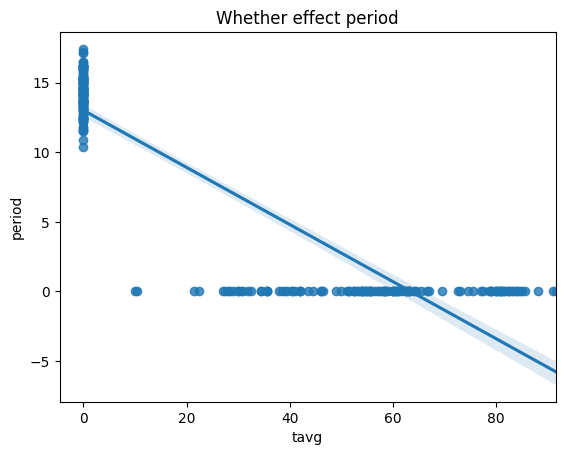
\includegraphics[width=0.5\textwidth]{plots/p7.png}
    % \includegraphics[width=\textwidth]{download.png}
    % this ensures your figures are centered where possible
    \caption{Weather Impact period} % refer to this image as (Figure 1)
    \label{fig:image3}
\end{figure}

\begin{figure}[!h]
    % change the scale multiplier to make the figures smaller or larger
    \centering
    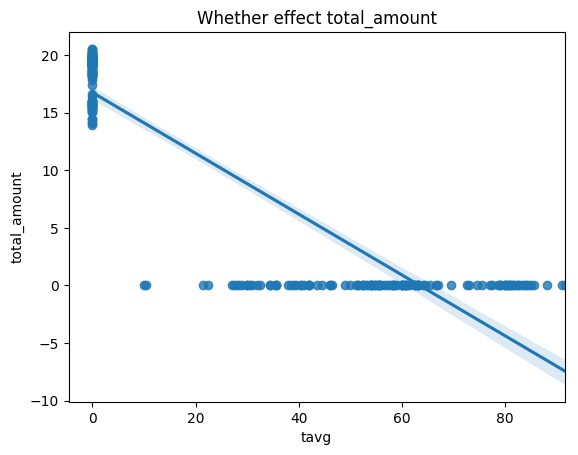
\includegraphics[width=0.5\textwidth]{plots/p8.png}
    % \includegraphics[width=\textwidth]{download.png}
    % this ensures your figures are centered where possible
    \caption{Weather Impact total amount} % refer to this image as (Figure 1)
    \label{fig:image3}
\end{figure}

From figure \ref{fig:image3} , We can draw the conclusion that the taxi bussiness get more tip and trip distance when the weather gets cold.

\subsubsection{Season affect}
In this section we shows that how the seasons affect the taxi bussiness. 
As shown in figure \ref{fig:image4}, The trip distance, tip amount doesn't change much through the seasons. The period and total amount get decrease in winter compare to the other seasons. 

\begin{figure}[!h]
    % change the scale multiplier to make the figures smaller or larger
    \centering
    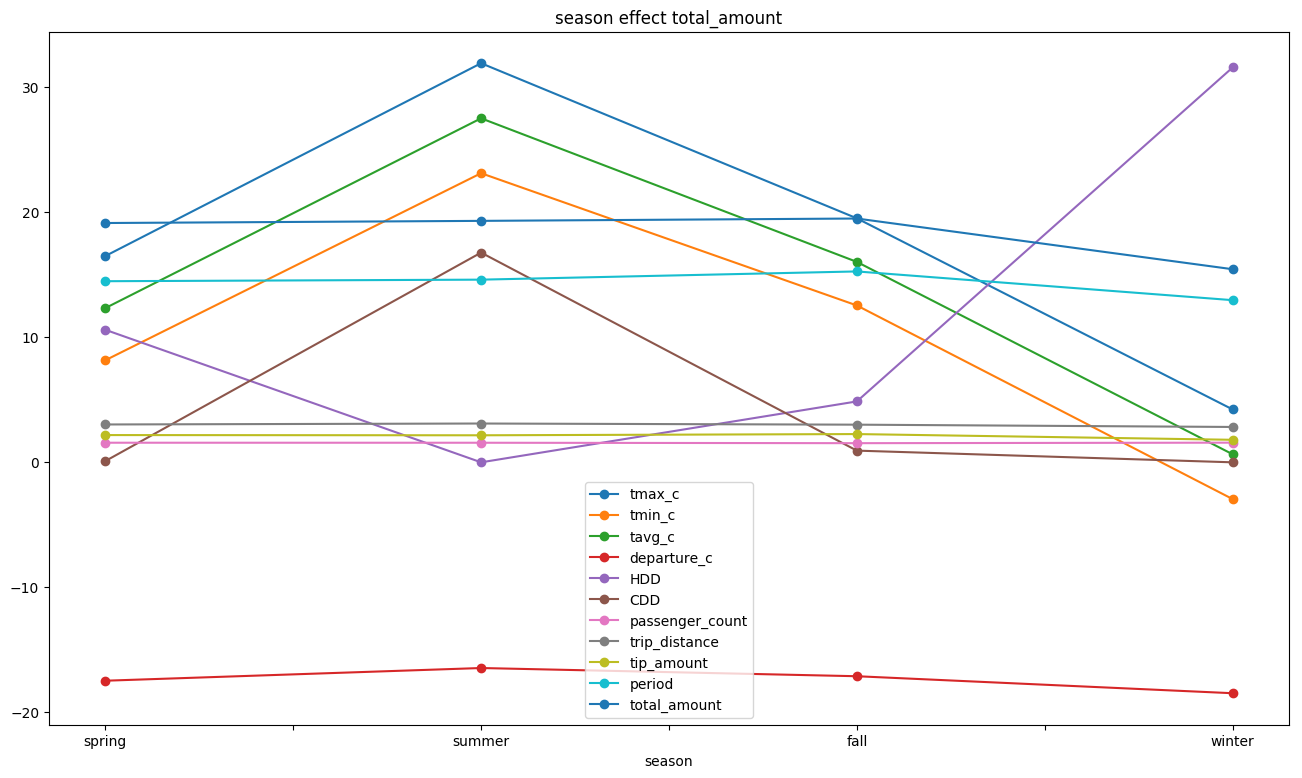
\includegraphics[width=0.8\textwidth]{plots/p9.png}
    % \includegraphics[width=\textwidth]{download.png}
    % this ensures your figures are centered where possible
    \caption{Season affect} % refer to this image as (Figure 1)
    \label{fig:image4}
\end{figure}


\section{Modelling}

In Modeling section we want to see which features contribute to the total\_amount feature. Since the total\_amount is the most important for taxi driver.

\subsection{Correlation Coefficient}
The correlation between attributes in the yellow taxi 2019year 4 months shown in figure \ref{fig:image9}, the features like 'trip\_distance', 'fare\_amount', 'tip\_amount', 'tolls\_amount', 'period' get high correlation scores of the total\_amount.

\begin{figure}[!h]
    % change the scale multiplier to make the figures smaller or larger
    \centering
    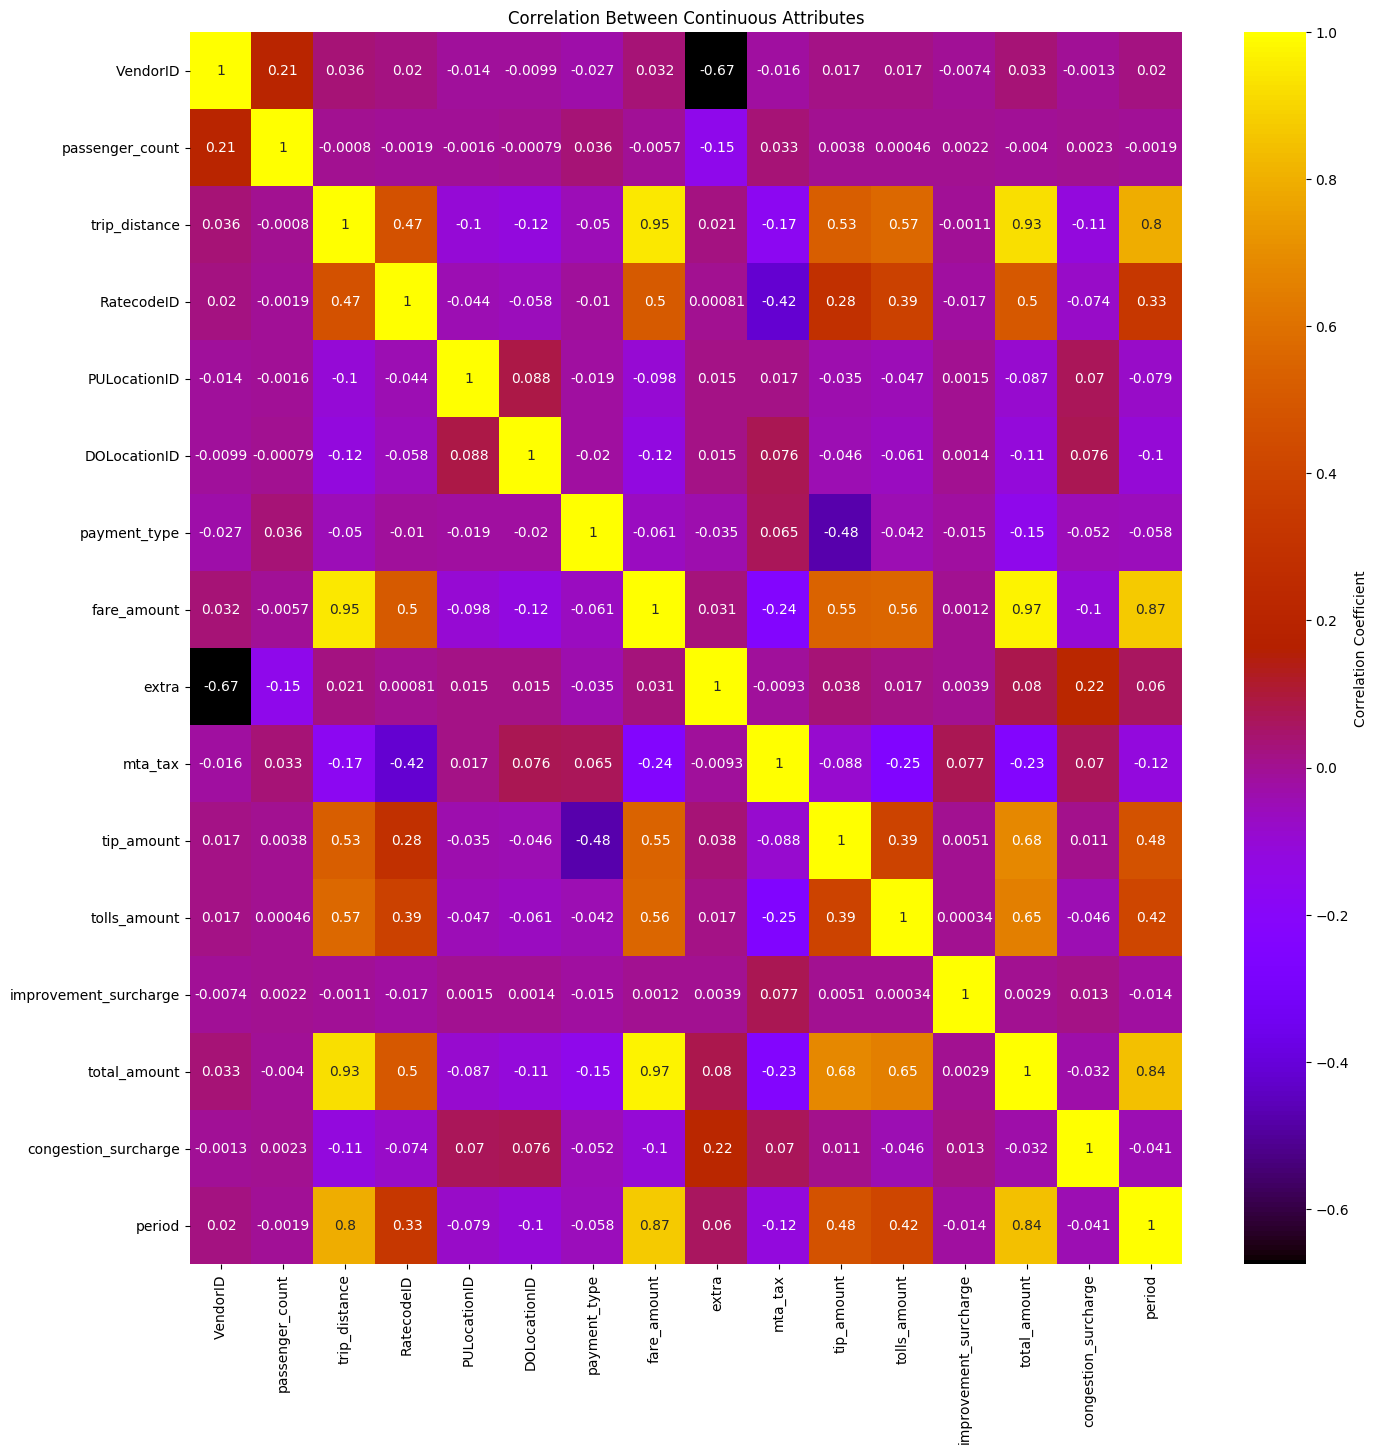
\includegraphics[width=0.8\textwidth]{plots/p10.png}
    % \includegraphics[width=\textwidth]{download.png}
    % this ensures your figures are centered where possible
    \caption{Correlation Coefficient} % refer to this image as (Figure 1)
    \label{fig:image9}
\end{figure}

\subsection{regression model}
The  total\_amount data feature will be predict using three regression models. They are linear regression model, Ridge regression model and Lasso regression model. According to the correlation heat map we created. We use feature 'trip\_distance', 'fare\_amount', 'tip\_amount', 'tolls\_amount', 'period' as our X feature. The y is of course the total\_amount.  The train-test split method is used to randomly split sampled data into 70\% training set and 30\% testing set.

\subsection{Evaluation and Results}

We evaluate the model by using Root Mean Square Error R2 score. The result is show in Table\ref{table1}.

\begin{table}[h]
    \centering  
    \caption{result table}  
    \label{table1} 
    %字母的个数对应列数,|代表分割线
    % l代表左对齐,c代表居中,r代表右对齐
    \begin{tabular}{|c|c|c|c|c|}  
        \hline  % 表格的横线
        & & & & \\[-6pt]  %可以避免文字偏上来调整文字与上边界的距离
        Model&Train RMSE&Test RMSE&Train R2&Test R2 \\  % 表格中的内容,用&分开,\\表示下一行
        \hline
        & & & & \\[-6pt]  %可以避免文字偏上 
        Linear&1.25&1.25&1.0& 1.0 \\
        Ridge&1.25&1.25&1.0& 1.0 \\
        Lasso&1.25&1.25&1.0& 1.0 \\
        \hline
    \end{tabular}
\end{table}

The coefficient of the three models are show:

\begin{figure}[!h]
    % change the scale multiplier to make the figures smaller or larger
    \centering
    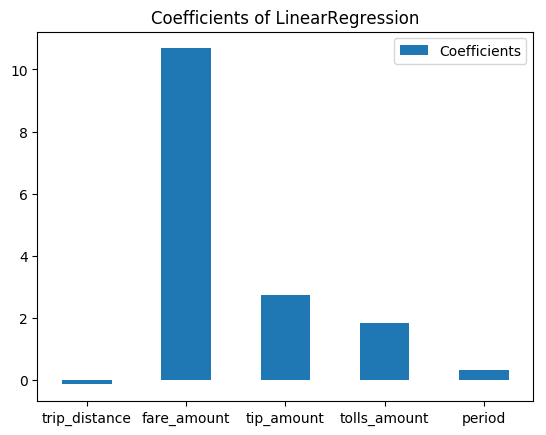
\includegraphics[width=0.7\textwidth]{plots/p11.png}
    % \includegraphics[width=\textwidth]{download.png}
    % this ensures your figures are centered where possible
    \caption{Linear} % refer to this image as (Figure 1)
    \label{fig:image4}
\end{figure}


\begin{figure}[!h]
    % change the scale multiplier to make the figures smaller or larger
    \centering
    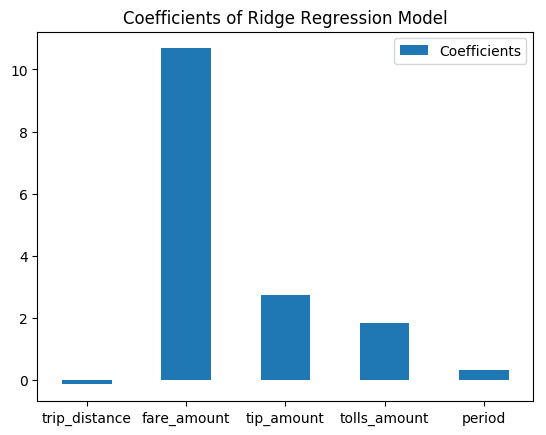
\includegraphics[width=0.7\textwidth]{plots/p12.png}
    % \includegraphics[width=\textwidth]{download.png}
    % this ensures your figures are centered where possible
    \caption{Ridge} % refer to this image as (Figure 1)
    \label{fig:image4}
\end{figure}


\begin{figure}[!h]
    % change the scale multiplier to make the figures smaller or larger
    \centering
    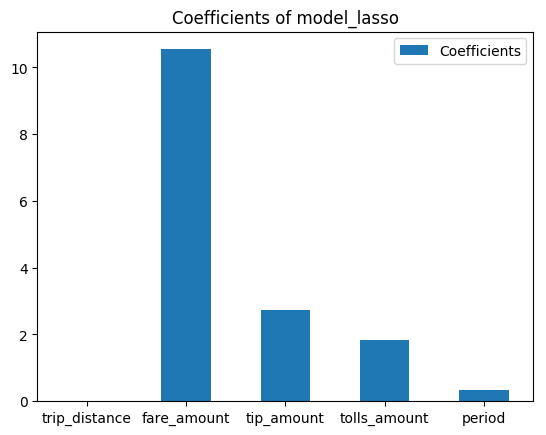
\includegraphics[width=0.7\textwidth]{plots/p13.png}
    % \includegraphics[width=\textwidth]{download.png}
    % this ensures your figures are centered where possible
    \caption{Lasso} % refer to this image as (Figure 1)
    \label{fig:image4}
\end{figure}


\subsection{Discussion}
As we can see of the three regression models, the fare\_amount features contribute to the final total\_amount most, since its coefficient is the biggest. We can indicate that the more fare\_amount the more total\_amount.

\section{Recommendations}
After all the analysis, we can learn that the weather affect the New York City taxi industry greatly. The colder the weather is the more people want to take taxi. But the cold day taxi trip distance is less than other season. In order for the taxi driver make more money the fare amount can take higher. 

\section{Conclusion}
In conclusion, after doing the exploratory analysis of yellow taxi trip records in 2019 4 months and combine with New York City Weather Data 2019 data. We learn much more about the New York City taxi industry. The visualisation help us taxi usage on different weather. We also build model to predict the total amount. The fare\_amount affect the total\_amount the most.

\clearpage

% BEGIN REFERENCES SECTION
\printbibliography



\end{document}
